\section{Auswertung}
\subsection{Magnetische Flußdichte einer Spule}

Zunächst wird das Magnetfeld einer langen Spule mit einer Hall-Sonde ausgemessen.
Die Messergebnisse sind in Abbildung (\ref{abb:7}) graphisch dargestellt und in der
Tabelle (\ref{tab:1}) tabellarisch. Das Magnetfeld dieser Spule wird von links und
von rechts seperat gemessen, da die Hall-Sonde nicht lang genug ist. Mithilfe
der Gleichung (\ref{eq:7}) wird die Theoriekurve bestimmt. Die Parameter der Spule lauten:

\begin{itemize}
  \item Windungszahl: n=300
  \item mittlerer Spulendurchmesser: d = \SI{0.041}{\meter}
  \item Spulenlänge: l = \SI{0.19}{\meter}
  \item Strom: I = \SI{1}{\ampere}
\end{itemize}

\begin{table}[H]
  \centering
  \caption{Messwerte des Magnetfeldes der langen Spule.}
  \label{tab:1}
  \begin{tabular}{c c}
    \toprule
    $x/\si{\meter}$ & $B/\si{\milli\tesla}$ \\
    \midrule
    0,01 & 0,409 \\
    0,02 & 0,732 \\
    0,03 & 1,276 \\
    0,04 & 1,801 \\
    0,05 & 2,098 \\
    0,06 & 2,237 \\
    0,07 & 2,305 \\
    0,08 & 2,338 \\
    0,09 & 2,355 \\
    0,10 & 2,363 \\
    0,11 & 2,366 \\
    0,12 & 2,362 \\
    0,13 & 2,349 \\
    0,14 & 2,252 \\
    0,15 & 2,213 \\
    0,16 & 2,151 \\
    0,17 & 2,030 \\
    0,18 & 1,755 \\
    0,19 & 1,275 \\
    0,20 & 0,707 \\
    0,21 & 0,354 \\
    \bottomrule
  \end{tabular}
\end{table}

\begin{figure}[H]
  \centering
  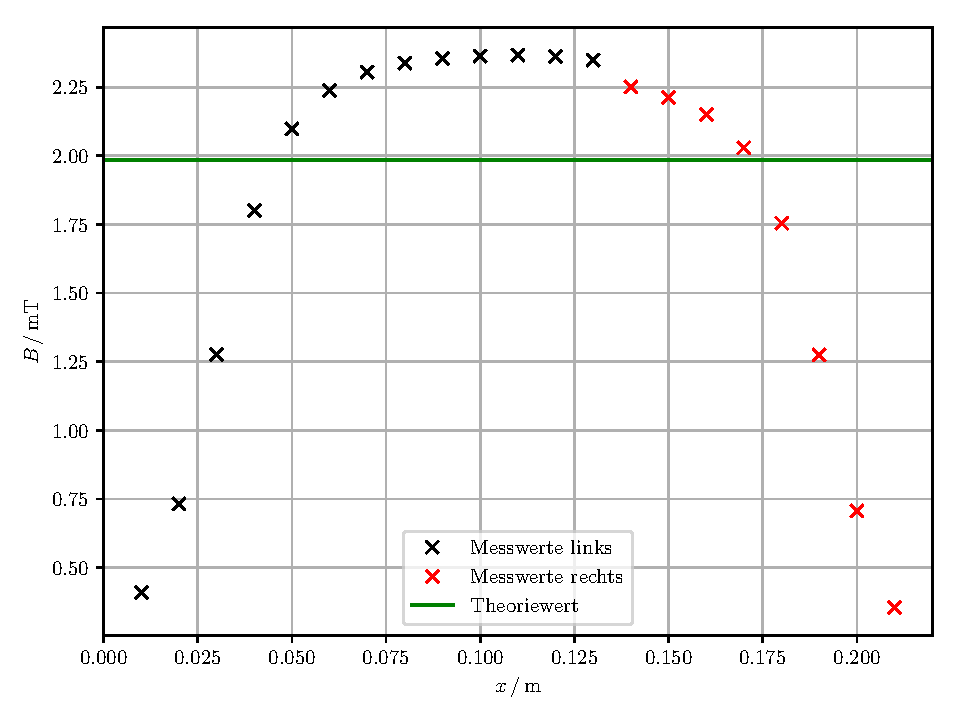
\includegraphics{plot1.pdf}
  \caption{Graphische Darstellung der Messwerte, die von links und von rechts Gemessen wurden.}
  \label{abb:7}
\end{figure}


Daraufhin wird das Magnetfeld einer kürzeren Spule untersucht. Die Messwerte sind in
Tabelle (\ref{tab:2}) und in Abbildung (\ref{abb:8}) dargestellt. Auch bei dieser
Spule werden die Theoriewerte mithilfe der Gleichung (\ref{eq:7}) bestimmt. Die
Parameter dieser Spule lauten wie folgt:

\begin{itemize}
  \item Windungszahl: n = 100
  \item mittlerer Spulendurchmesser: d = \SI{0.041}{\meter}
  \item Spulenlänge: l = \SI{0.085}{\meter}
  \item Strom: I = \SI{1}{\ampere}
\end{itemize}

\begin{table}[H]
  \centering
  \caption{Messwerte des Magnetfeldes der kurzen Spule.}
  \label{tab:2}
  \begin{tabular}{c c}
    \toprule
    $x/\si{\meter}$ & $B/\si{\milli\tesla}$ \\
    \midrule
    0,01  & 0,144 \\
    0,015 & 0,211 \\
    0,02  & 0,321 \\
    0,025 & 0,470 \\
    0,03  & 0,677 \\
    0,035 & 0,940 \\
    0,04  & 1,225 \\
    0,045 & 1,468 \\
    0,05  & 1,664 \\
    0,055 & 1,781 \\
    0,06  & 1,840 \\
    0,065 & 1,853 \\
    0,07  & 1,816 \\
    0,075 & 1,736 \\
    0,08  & 1,580 \\
    0,085 & 1,371 \\
    0,09  & 1,071 \\
    0,095 & 0,806 \\
    0,10  & 0,570 \\
    0,105 & 0,393 \\
    0,11  & 0,259 \\
    0,115 & 0,180 \\
    0,12  & 0,115 \\
    \bottomrule
  \end{tabular}
\end{table}

\begin{figure}[H]
  \centering
  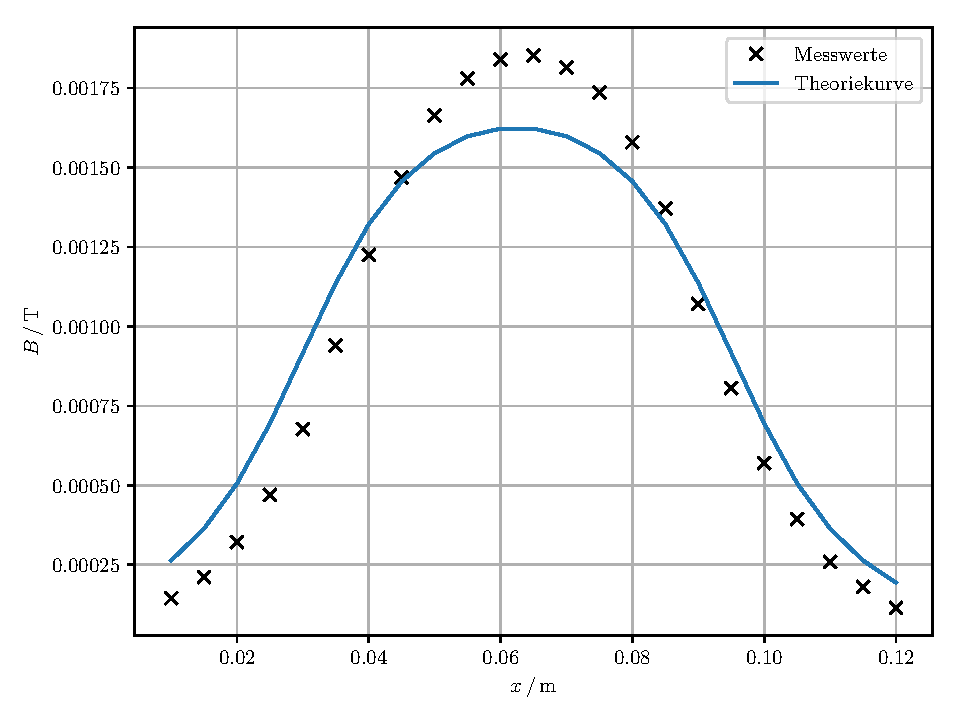
\includegraphics{plot2.pdf}
  \caption{Graphische Darstellung der Messwerte für die kurze Spule.}
  \label{abb:8}
\end{figure}

\subsection{Magnetfeld einer Helmholtz-Spule}

In dem zweiten Teil des Versuches wird nun das Magnetfeld einer Helmholz-Spule mit
verschiedenen Abständen der Spule ermittelt. Die Parameter des Spulenpaares lauten:

\begin{itemize}
  \item Windungszahl pro Spule: n = 100
  \item mittlerer Spulendurchmesser: d = \SI{1.25}{\meter}
  \item Spulenbreite: b = \SI{0.033}{\meter}
  \item Strom: I = \SI{3}{\ampere}
\end{itemize}

Der erste Abstand der beiden Spulen ist \SI{0.07}{\meter}. Für diesen Fall sind
die Messergebnisse in Tabelle (\ref{tab:3}) und in der Abbildung (\ref{abb:9})
dargestellt.

\begin{table}[H]
  \centering
  \caption{Messwerte der Helmholz-Spule für den Abstand \SI{0.07}{\meter}.}
  \label{tab:3}
  \begin{tabular}{c c}
    \toprule
    $x/\si{\centi\meter}$ & $B/\si{\milli\tesla}$ \\
    \midrule
     0,8 & 3,757 \\
     1,0 & 3,758 \\
     1,2 & 3,761 \\
     1,4 & 3,762 \\
     1,6 & 3,764 \\
     1,8 & 3,765 \\
     2,0 & 3,767 \\
     2,2 & 3,767 \\
     2,4 & 3,762 \\
     7,6 & 2,756 \\
     8,0 & 2,607 \\
     8,4 & 2,419 \\
     8,8 & 2,241 \\
     9,2 & 2,066 \\
     9,6 & 1,911 \\
    10,0 & 1,756 \\
    10,4 & 1,613 \\
    10,8 & 1,481 \\
    11,2 & 1,358 \\
    11,6 & 1,240 \\
    12,0 & 1,143 \\
    12,4 & 1,042 \\
    12,8 & 0,955 \\
    13,2 & 0,869 \\
    13,6 & 0,798 \\
    14,0 & 0,740 \\
    14,4 & 0,672 \\
    14,8 & 0,618 \\
    15,2 & 0,574 \\
    15,6 & 0,525 \\
    16,0 & 0,487 \\
    \bottomrule
  \end{tabular}
\end{table}

\begin{figure}[H]
  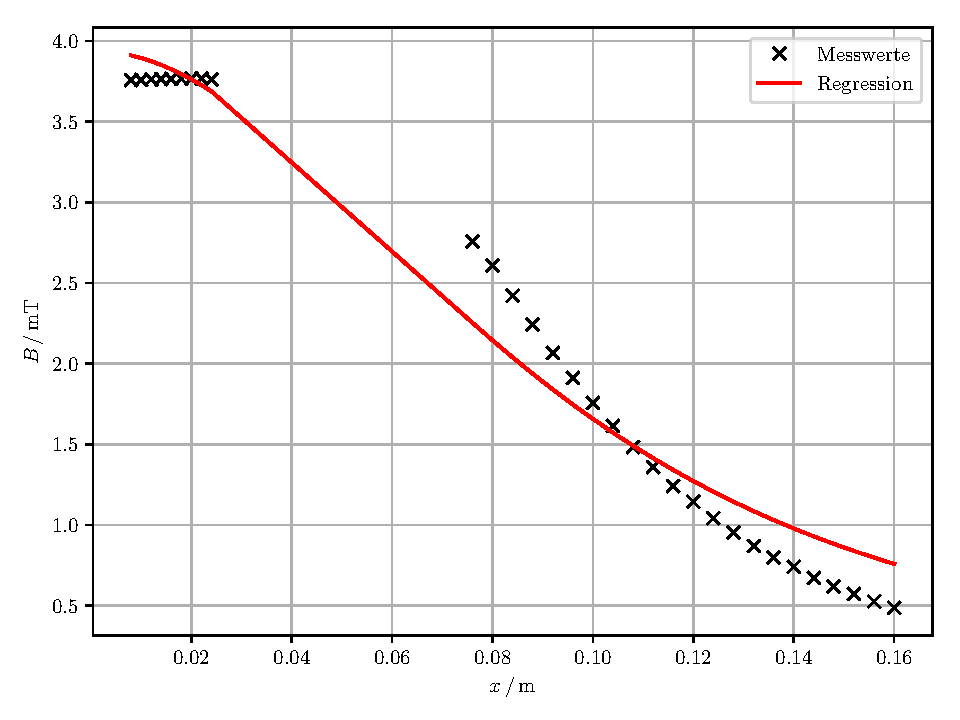
\includegraphics{plot3.pdf}
  \caption{Graphische Darstellung der Messwerte für das Spulenpaar bei \SI{0.07}{\meter}.}
  \label{abb:9}
\end{figure}

Der nächste Abstand der beiden Spulen ist \SI{0.1}{\meter}. Auch in diesem Fall
werden die Messwerte in der Tabelle (\ref{tab:4}) und Abbildung (\ref{abb:10}) dargestellt.

\begin{table}[H]
  \centering
  \caption{Messwerte des Spulenpaares mit dem Abstand \SI{0.1}{\meter}.}
  \label{tab:4}
  \begin{tabular}{c c}
    \toprule
    $x/\si{\centi\meter}$ & $B/\si{\milli\tesla}$ \\
    \midrule
     0,8 & 3,031 \\
     1,0 & 3,009 \\
     1,2 & 2,985 \\
     1,4 & 2,959 \\
     1,6 & 2,937 \\
     1,8 & 2,918 \\
     2,0 & 2,902 \\
     2,2 & 2,888 \\
     2,4 & 2,878 \\
     2,6 & 2,870 \\
     2,8 & 2,865 \\
     3,0 & 2,864 \\
     3,2 & 2,866 \\
     3,4 & 2,871 \\
     3,6 & 2,879 \\
     3,8 & 2,891 \\
     4,0 & 2,907 \\
     4,2 & 2,927 \\
     4,4 & 2,945 \\
     4,6 & 2,968 \\
     4,8 & 2,995 \\
     5,0 & 3,015 \\
     5,2 & 3,045 \\
     5,4 & 3,062 \\
    10,8 & 2,475 \\
    11,8 & 2,093 \\
    12,8 & 1,735 \\
    13,8 & 1,376 \\
    14,8 & 1,095 \\
    15,8 & 0,878 \\
    16,8 & 0,707 \\
    17,8 & 0,568 \\
    18,8 & 0,459 \\
    19,8 & 0,375 \\
    20,8 & 0,310 \\
    21,8 & 0,260 \\
    22,8 & 0,217 \\
    23,8 & 0,182 \\
    24,8 & 0,159 \\
    \bottomrule
  \end{tabular}
\end{table}

\begin{figure}[H]
  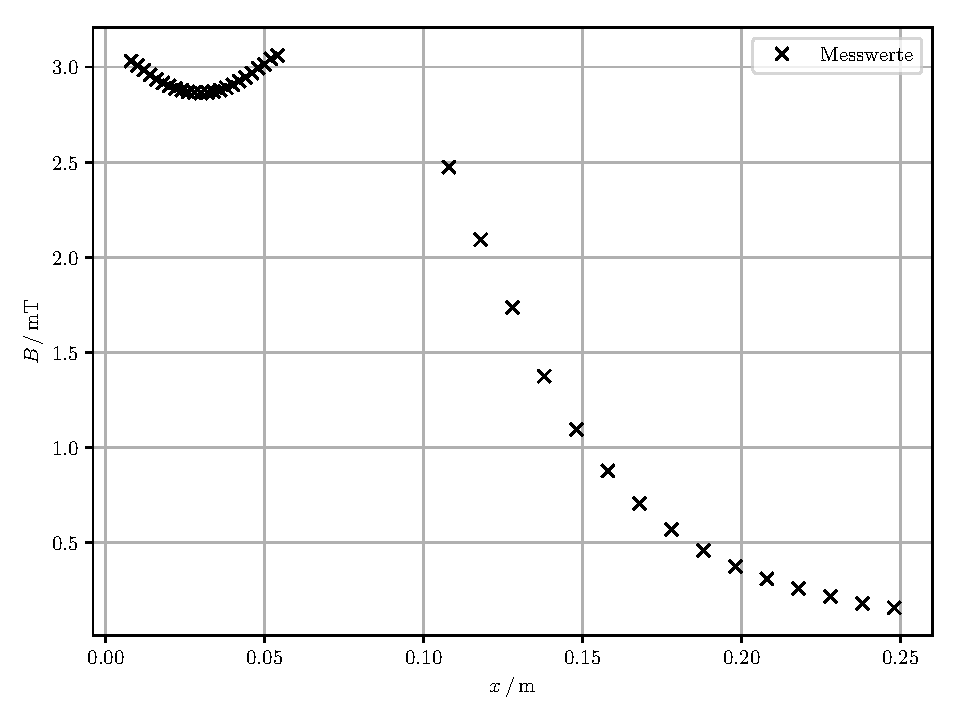
\includegraphics{plot4.pdf}
  \caption{Graphische Darstellung der Messwerte des Spulenpaares für den Abstand \SI{0.1}{\meter}.}
  \label{abb:10}
\end{figure}

Als letztes wird eine Helmholz-Spule mit dem Abstand \SI{0.14}{\meter} untersucht.
Die Messwerte des Magnetfeldes werden in der Tabelle (\ref{tab:5}) und in der Abbildung
(\ref{abb:11}) dargestellt.

\begin{table}[H]
  \centering
  \caption{Messwerte des Spulenpaares mit dem Abstand \SI{0.14}{\meter}.}
  \label{tab:5}
  \begin{tabular}{c c}
    \toprule
    $x/\si{\centi\meter}$ & $B/\si{\milli\tesla}$ \\
    \midrule
    0,8 & 2,517 \\
    1,3 & 2,411 \\
    1,8 & 2,288 \\
    2,3 & 2,156 \\
    2,8 & 2,056 \\
    3,3 & 1,969 \\
    3,8 & 1,903 \\
    4,3 & 1,855 \\
    4,8 & 1,835 \\
    5,3 & 1,837 \\
    5,8 & 1,866 \\
    6,3 & 1,915 \\
    6,8 & 1,985 \\
    7,3 & 2,101 \\
    7,8 & 2,179 \\
    8,3 & 2,316 \\
    8,8 & 2,440 \\
    9,3 & 2,571 \\
    15  & 2,233 \\
    16  & 1,891 \\
    17  & 1,557 \\
    18  & 1,240 \\
    19  & 1,005 \\
    20  & 0,796 \\
    21  & 0,636 \\
    22  & 0,513 \\
    23  & 0,414 \\
    24  & 0,344 \\
    25  & 0,282 \\
    \bottomrule
  \end{tabular}
\end{table}

\begin{figure}[H]
  \centering
  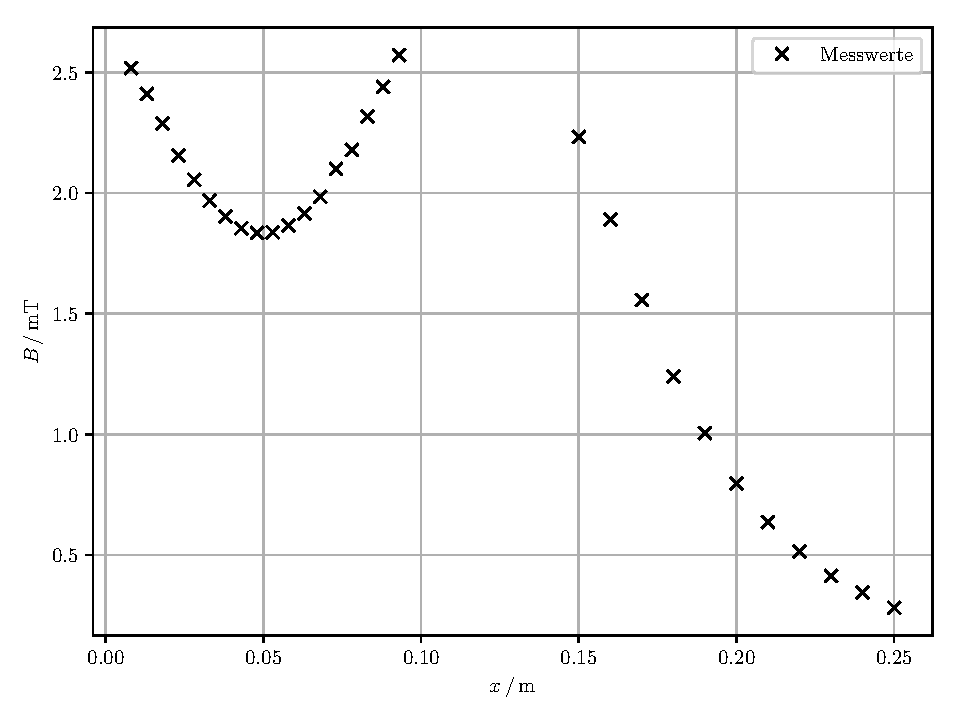
\includegraphics{plot5.pdf}
  \caption{Graphische Darstellung der Messwerte des Spulenpaares für den Abstand \SI{0.14}{\meter}.}
  \label{abb:11}
\end{figure}

\subsection{Bestimmung der Hysteresekurve}

In dem letzten Teil wird nun die Hysteresekurve eines Materials bestimmt. Dafür werden
die Messwerte Graphisch in der Abbildung (\ref{abb:12}) dargestellt um die Parameter
der Kurve zu bestimmen.

\begin{table}
  \centering
  \caption{Messwerte der Neukurve.}
  \label{tab:6}
  \begin{tabular}{c c}
    \toprule
    $I/\si{\ampere}$ & $B/\si{\milli\tesla}$ \\
    \midrule
    1  &  98,1 \\
    2  & 257,5 \\
    3  & 380,0 \\
    4  & 468,2 \\
    5  & 528,2 \\
    6  & 572,4 \\
    7  & 609,8 \\
    8  & 641,1 \\
    9  & 668,6 \\
    10 & 694,2 \\
    \bottomrule
  \end{tabular}
\end{table}

\begin{table}
  \centering
  \caption{Messwerte für die Hysteresekurve.}
  \label{tab:7}
  \begin{tabular}{c c| c c| c c|c c}
    \toprule
    $I/\si{\ampere}$ & $B/\si{\milli\tesla}$ & $I/\si{\ampere}$ & $B/\si{\milli\tesla}$& $I/\si{\ampere}$ & $B/\si{\milli\tesla}$& $I/\si{\ampere}$ & $B/\si{\milli\tesla}$ \\
    \midrule
    10    & 694,2 & 0     & 56,5 &-9,5  &-680,1&0     &-106,0   \\
    9,5   & 683,4 & -0,5  & 20,2 &-9    &-672,2&0,5   & -29,6  \\
    9     & 675,1 & -1    & -76,8&-8,5  &-663,5&1     &  64,2   \\
    8,5   & 666,7 & -1,5  &-160,2&-8    &-653,6&1,5   & 151,8   \\
    8     & 656,7 & -2    &-241,7&-7,5  &-644,0&2     & 239,7   \\
    7,5   & 647,1 & -2,5  &-313,7&-7    &-632,8&2,5   & 311,6   \\
    7     & 636,5 & -3    &-370,0&-6,5  &-621,6&3     & 371,8   \\
    6,5   & 625,0 & -3,5  &-422,5&-6    &-608,5&3,5   & 430,8   \\
    6     & 612,4 & -4    &-460,2&-5,5  &-595,3&4     & 460,0   \\
    5,5   & 598,7 & -4,5  &-495,9&-5    &-580,2&4,5   & 495,0   \\
    5     & 583,1 & -5    &-521,8&-4,5  &-564,0&5     & 523,5   \\
    4,5   & 566,7 & -5,5  &-546,1&-4    &-544,9&5,5   & 547,3   \\
    4     & 548,0 & -6    &-568,2&-3,5  &-522,9&6     & 568,2   \\
    3,5   & 526,9 & -6,5  &-588,2&-3    &-497,6&6,5   & 587,0   \\
    3     & 502,8 & -7    &-605,2&-2,5  &-470,9&7     & 605,8   \\
    2,5   & 472,1 & -7,5  &-622,2&-2    &-434,1&7,5   & 623,8   \\
    2     & 436,9 & -8    &-636,9&-1,5  &-383,1&8     & 635,9   \\
    1,5   & 386,8 & -8,5  &-651,3&-1    &-318,3&8,5   & 650,6   \\
    1     & 308,3 & -9    &-664,6&-0,5  &-211,3&9     & 664,1   \\
    0,5   & 212,0 & -9,5  &-676,9&0     &-123,4&9,5   & 675,9   \\
    0     & 126,5 & -10   &-688,4& - & -       &10    & 687,7   \\
    \bottomrule
  \end{tabular}
\end{table}

\begin{figure}[H]
  \centering
  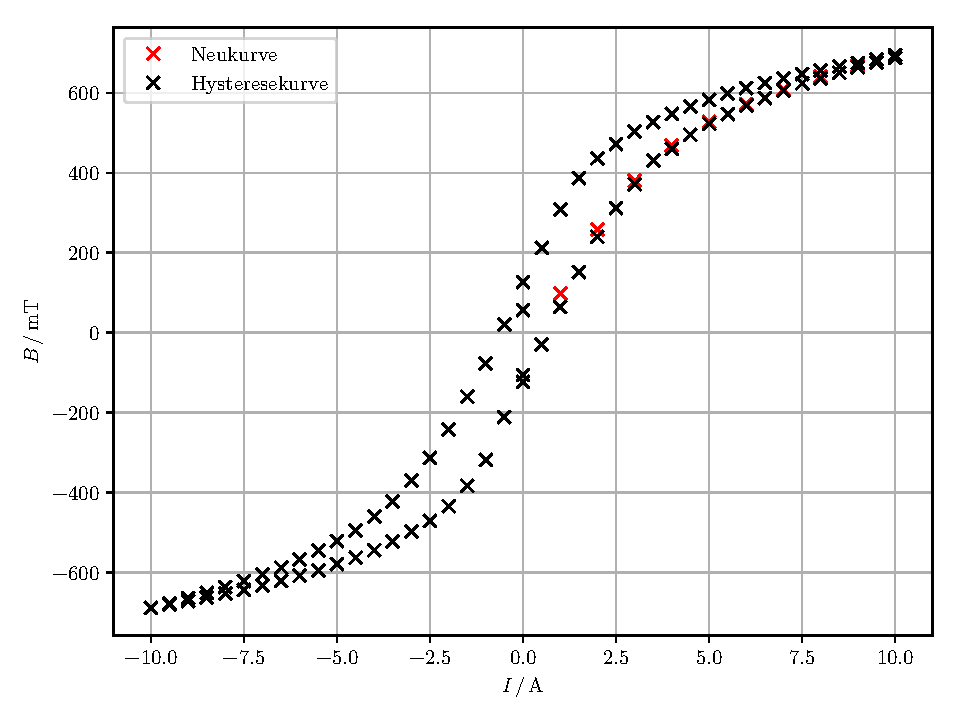
\includegraphics{plot6.pdf}
  \caption{Graphische Darstellung der Hysteresekurve.}
  \label{abb:12}
\end{figure}

Aus dem Graphen lässt sich nun die Sättigungsmagnetisierung, die Remanenz und die
Koerzitivkraft bestimmen.

Die Sättigungsmagnetisierung kann nur näherungsweise bestimmt werden, da die
maximale Spannung des Generators \SI{10}{\volt} ist und sich bei dieser Spannung noch
keine Sättigungsmagnetisierung einstellt. Näherungsweise ist die Sättigungsmagnetisierung
damit

\begin{equation*}
  B_s = \SI{694.2}{\milli\tesla}.
\end{equation*}

Auch die Remanenz lässt sich aus dem Graphen ablesen. Da nicht genau gemessen werden
kann muss der Mittelwert und die Standardabweichung aus den zwei möglichen Werten der Remanenz bestimmt werden
mit folgenden Formeln.

\begin{equation}
    \bar{x} = \frac{1}{N} \sum_{i=1}^{N} x_i
\end{equation}

\begin{equation}
  \Delta \bar{x} = \frac{1}{\sqrt{N}\sqrt{N-1}} \sqrt{\sum_{i}(x_i-\bar{x})^2}
\end{equation}

Damit ergibt sich die Remanenz zu:

\begin{equation*}
  B_r = \SI{91.5(350)}{\milli\tesla}
\end{equation*}

Für die Koerzitivkraft wird wieder der Graph der Hysteresekurve betrachtet. Die
Koerzitivkraft ist in diesem Fall als Strom angegeben, der für das Magnetfeld der
Spule verantwortlich ist. Die Koerzitivkraft ist somit:

\begin{equation*}
  I_c = \SI{-0.6}{\ampere}
\end{equation*}
